%--------------------------------------------------------------------------------------------------
\chapter{Stand der Technik}\label{cha:StandDerTechnik}

In diesem Kapitel gibt es einen Einblick in die drei Themenbereiche Industrie 4.0, industrielle Fertigung, Mensch-Computer Interaktion und Virtual Reality.  TODO
\newline\newline
Daher werden wir uns zunächst mit dem Begriff Industrie 4.0 auseinander setzen, den Begriff definieren und auf die Geschichte der Industriellen Revolutionen der vergangenen 260 Jahre sowie auf die Veränderungen in der Informations- und Kommunikationstechnik eingehen. Daraufhin gibt es einen Einblick in die Potentiale und Herausforderungen von Industrie 4.0. Zum Abschluss dieses Abschnittes werden verschiedene Leitfaden zur Umsetzung von Industrie 4.0 für Unternehmen vorgestellt.
\newline\newline
Daraufhin gib es einen Einblick in die Ausgangslage der industriellen Fertigung, insbesondere in den Produktlebenszyklus, die Automatisierungspyramide und TODO
\newline\newline
Als nächstes setzen wir uns auseinander mit dem Thema Mensch-Computer Interaktion (HCI). Dazu gibt es einen Einblick in die Geschichte der HCI der Vergangenen [XXX] Jahre, bevor wir aktuelle Entwicklungen in dem Bereich vorgestellt werden.
\newline\newline
Zum Schluss wird das Thema Virtual Reality (VR) vorgestellt und es gibt einen Einblick in die Geschichte, den Stand der Technik und technische Herausforderungen von Virtual Reality. Daraufhin werden vielversprechende Entwicklungen für die Zukunft von Virtual Reality vorgestellt.


%--------------------------------------------------------------------------------------------------
\section{Industrie 4.0}\label{sec:Industrie4.0}
Erstmalig tauchte der Begriff Industrie 4.0 auf der Hannover Messe 2011 auf und wurde daraufhin ein zentraler Bestandteil der Hightech-Strategie der deutschen Bundesregierung [8, BDI, Einblick i.d.4.Rev].
\newline
Der Begriff Industrie 4.0 „steht für die 4. Industrielle Revolution, einer neuen Stufe der Organisation und Steuerung der gesamten Wertschöpfungskette über den Lebenszyklus von Produkten“ [1, Anderl, Vortrag 2015]. Dies führt zum einem zu einer zunehmenden Vernetzung von „Mensch, Maschinen und Werkstücken durch Modernste Informations- und Kommunikationstechnik“ [6, BDI, Was ist Industrie 4.0], zum anderen auch zu einer zunehmenden „Vernetzung der realen mit der virtuellen Welt“ [7, DIN, Def. Ind.4]. Grundlage dieser Wandlung in der Industrie sind sogenannte Cyber-Physische-Systeme (CPS), also moderne Steuerungssysteme mit eingebetteten Softwaresystemen und Anbindung an das Internet [1, Anderl, Vortrag 2015]. Cyber-Physische-Systeme verknüpfen „reale (physische) Objekte und Prozesse mit informationsverarbeitenden (virtuellen) Objekten und Prozessen“ [11, Fraunhofer, CPS]. Die hat eine zunehmende Verschmelzung von Fertigungsprozessen und Informationstechnologie zur Folge [7, DIN, Def. Ind.4].

\subsection{Industrielle Revolution und Informations- und Kommunikationstechnik}\label{sec:GeschichteIndustrie4}

Um den Begriff Industrie 4.0 besser nachvollziehen zu können, ist es unumgänglich die Geschichte der industriellen Revolutionen der vergangenen 260 Jahre zu verstehen. Der Begriff Industrie 4.0 „leitet sich aus den großen Industriegeschichtlichen Umbrüchen ab“ [7, DIN, Def. Ind.4] und ist ein Wortspiel aus den Anteilen „Industrie“ und „4.0“. Der Anteil „4.0“ soll zum einem eine Assoziation zum Internet (Web 4.0) herstellen und zum anderen, wie in der heutigen Zeit üblich eine Versionsbezeichnung darstellen, wie man sie aus dem Bereich der Softwareentwicklung kennt [1, Anderl, Vortrag 2015].
\newline
Industrie 4.0 wird als „der vierte große Technologische Durchbruch“ [7, DIN, Def. Ind.4] betrachtet. Daher werden im Folgenden die industriellen Revolutionen bis zur Industrie 4.0 und die Entwicklung der Informations- und Kommunikationstechnik bis zu Web 4.0 betrachtet.

\subsubsection{Die industriellen Revolutionen}\label{sec:IndustrielleRevolution}
\begin{figure}[h]
	\centering
	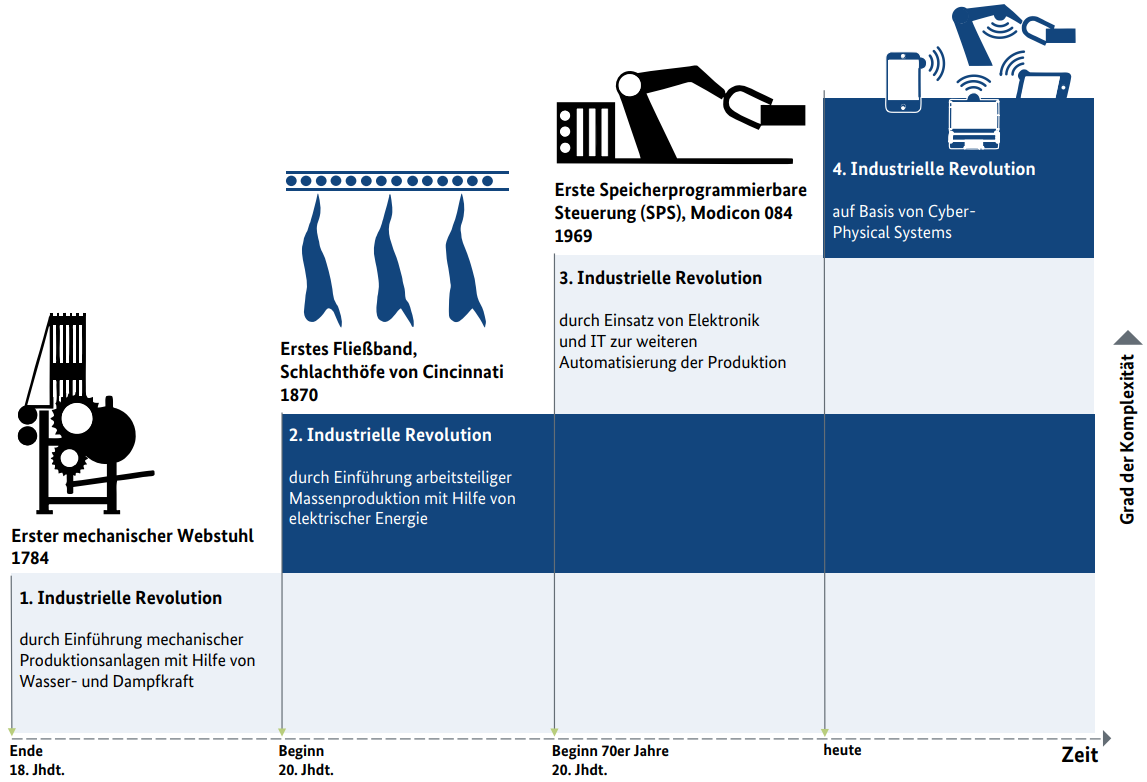
\includegraphics[width=1\linewidth]{Bilder/A1_DieGeschichteDerIndustriellenRevolutionenBMWI}
	\caption{Die Geschichte der Industriellen Revolutionen [A1, BMWi, S.8]}
	\label{fig:IndustrielleRevolutionenBild}
\end{figure}
Die \textbf{erste industrielle Revolution} spielte sich Mitte bis Ende des 18. Jahrhunderts ab. Im Fokus standen Wasser- und Dampfkraft, was die Möglichkeit mit sich brachte, Maschinen die vorher noch mit menschlicher Kraft angetrieben wurden, mithilfe von Wasser- und Dampfkraft anzutreiben. Die Menschen erkannten früh, dass sich durch die neuen industriellen Entwicklungen eine große Menge an Arbeitsplätzen schaffen lassen können. [9, Industrie Wegweiser, Ind.Wandel d.Z.]. Neben gesteigerter Produktivität in der Herstellung führte die erste industrielle Revolution dazu, „dass seit dieser Zeit in industriell geprägten Ländern keine strukturell bedingten Hungerkatastrophen mehr entstanden sind“ [B1, Bauernhansl, S.5]. Des Weiteren führte die verbesserte Infrastruktur durch Dampfschiffe und Eisenbahnen zu einer besseren Kleidungs- und Nahrungsversorgung und zu einem enormen Bevölkerungswachstum [B1, Bauernhansl, S.5]. Außerdem gab es große Auswirkungen auf die Gesellschaft, da zwei neue Schichten in der Bevölkerung entstanden: Die Fabrikarbeiterschaft und die Fabrikbesitzer. [B1, Bauernhansl, S.5]. Die Entwicklungen der ersten industriellen Revolution brachten allerdings einige große Probleme mit sich. Dazu gehören Beispielsweise die Ausbeutung der Fabrikmitarbeiter durch schlechte Arbeitsbedingungen und Bezahlung, Kinderarbeit und sogar eine verkürzte Lebenserwartung für die Fabrikmitarbeiter [B1, Bauernhansl, S.5].
\newline\newline
Die \textbf{zweite industrielle Revolution} zu Beginn des 20. Jahrhunderts „war geprägt durch Arbeitsteilige Massenproduktion mit Hilfe elektrischer Energie“ [B1, Bauernhansl, S.5]. Ermöglicht wurde die Massenproduktion unter anderem durch das von Henry Ford entwickelte Fließband, welches bereits 1913 in der Automobilproduktion eingesetzt wurde [10, Spiegel, Industrielle Revolutionen].Des Weiteren führten die Entwicklungen von elektrischen Antrieben und Verbrennungsmotoren zu einer zunehmenden Dezentralisierung. Dezentralisierung im Kontext der zweiten industriellen Revolution bedeutet, „die Arbeitsmaschinen nicht durch zentrale Kraftmaschinen anzutreiben, sondern dezentral zu betreiben“ [B1, Bauernhansl, S.5]. Ein weiterer „Erfolgsfaktor in der zweiten Industriellen Revolution waren die ersten Schritte der Globalisierung“ [9, Industrie Wegweise, I.i.W.d.Z.] durch die Fortschritte in der Verkehrsinfrastruktur. Dazu gehören Beispielsweise moderne Schiffe, die eine bessere Vernetzung zwischen den Kontinenten ermöglicht haben [9, Industrie Wegweise, I.i.W.d.Z.]. Für die Chemie- und Automobilindustrie wurde Erdöl zu einem wichtigen Rohstoff. „Die Großindustrielle Massenproduktion“ [B1, Bauernhansl, S.5] ermöglichte die Produktion von immer günstigeren (Konsum-)Gütern für die weiterhin wachsende Bevölkerung [B1, Bauernhansl, S.5]. Die Gesellschaft erkannte, dass die Ausbeutung der Fabrikarbeiter nicht weiter gehen kann und Gewerkschaften gewannen stark an Bedeutung. Daher sollten Fabrikarbeiter von nun an besser entlohnt werden, um weitere Soziale Spannungen zu vermeiden [B1, Bauernhansl, S.5]. Im Übergang zwischen der ersten und zweiten industriellen Revolution zum verbreiteten sich die Ideen des Kommunismus und der Sozialdemokratie [B1, Bauernhansl, S.5].
\newline\newline
Die \textbf{dritte industrielle Revolution} Mitte des 20. Jahrhunderts wurde geprägt zunehmende Automatisierung der Produktionsabläufe durch das einbinden von Elektronik und Informations- und Kommunikationstechnik [B1, Bauernhansl, S.7]. Durch den Einsatz von programmierbaren Steuerungen, „waren auch in den Fabriken Programmierer gefragt“ [10, Spiegel, Industrielle Revolutionen]. Des Weiteren wurde der Personal-Computer (PC) vermehrt im Büro aber auch im Haushalt eingesetzt [9, Industrie Wegweise, I.i.W.d.Z.]. Die Entwicklungen der dritten industriellen Revolution ermöglichten eine variantenreiche Serienproduktion. Mit dieser Entwicklung veränderten sich aber auch die Erwartungen der Kunden, welche nun vermehrt auf Individualität und Qualität der Produkte achteten [B1, Bauernhansl, S.7].
\newline\newline
Die \textbf{vierte industrielle Revolution} ist momentan noch im Gange. In Kapitel \ref{sec:PotentialeIndustrie4.0} und \ref{sec:HerausforderungenUmsetzung} gibt es einen Einblick in die Potentiale und Herausforderungen von Industrie 4.0. Vorweg lässt sich aber sagen, dass die vierte Industrielle Revolution die Industrie flexibler gestalten soll, statt ein höheres grad an Automatisierung zu erreichen. Die Wertschöpfung soll durch Cyber-Physische-Systeme verbessert werden. Es ist wichtig zu wissen, dass die Entwicklungen der Industrie 4.0 aus zwei Entwicklungsrichtungen kommen [1, Anderl, Vortrag 2015].
\begin{description}
	\item[1. Physicalize the Cyber] Aus der Sicht der Informationstechnischen Unternehmen: „Zunehmende Nutzung von Informationstechnik in der Produktion“ [1, Anderl, Vortrag 2015].
	\item[2. Cyberize the Physical] Aus der Sicht der Produktionstechnischen Unternehmen: „Anwendungen für Informationstechnik in der Produktion“ [1, Anderl, Vortrag 2015].
\end{description}

\subsubsection{Informations- und Kommunikationstechnik}\label{sec:WebRevolution}
\begin{figure}[h]
	\centering
	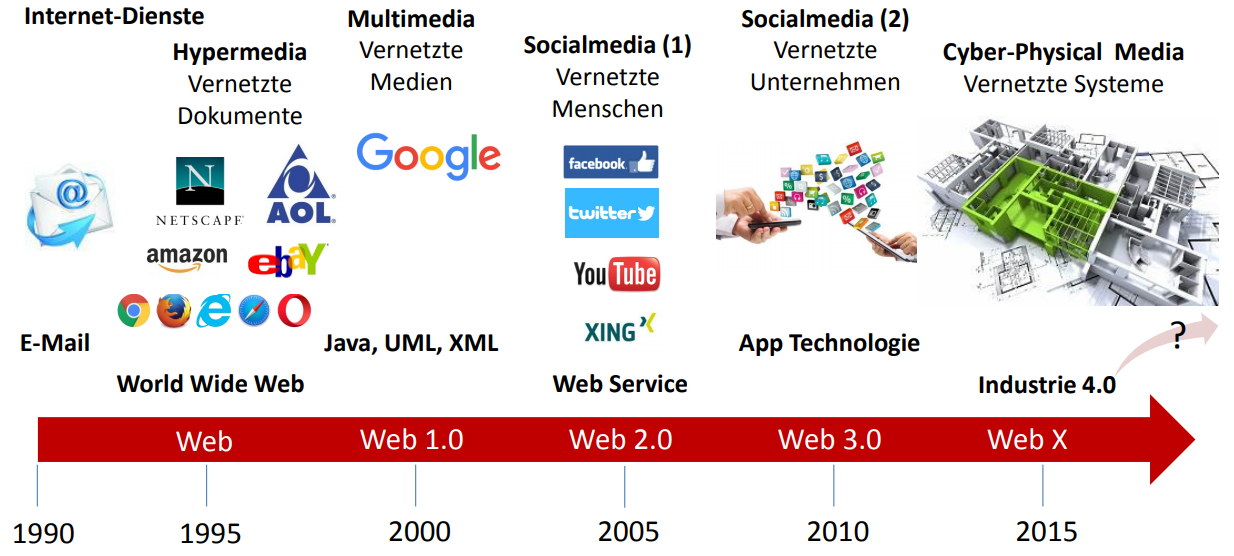
\includegraphics[width=1\linewidth]{Bilder/A2_EntwicklungWeb0-4}
	\caption{Die Entwicklung von Web bis Web 4.0 [A2, Kompet. Dig.Handwerk, S.3]}
	\label{fig:WebRevolutionBild}
\end{figure}
Genauso wie in der Industrie gab es in der Informations- und Kommunikationstechnik einige technologische Umbrüche. Auffällig ist, dass die sich die Technologien in der Informations- und Kommunikationstechnik im Vergleich zu den Fortschritten in der Industrie sehr schnell weiterentwickeln. Die wichtigsten Umbrüche sind in der Abbildung \ref{fig:WebRevolutionBild} zusammengefasst.
\newline\newline
Das wichtigste was man der Abbildung \ref{fig:WebRevolutionBild} entnehmen kann ist, dass in der neuen Entwicklungsstufe von Informations- und Kommunikationstechnik Cyber-Physische Medien im Mittelpunkt stehen.

\subsection{Potentiale von Industrie 4.0}\label{sec:PotentialeIndustrie4.0}

„Industrie 4.0 macht die Produktion individueller und effizienter“ [6, BDI, Was ist Industrie 4.0], und verspricht dem Wirtschaftsstandort Deutschland Wachstumschancen und sogar Wettbewerbsvorteile bei entsprechender Umsetzung. Laut dem Bundesverband der Deutschen Industrie (BDI) prognostizieren Experten eine Produktivitätssteigerung von bis zu 30 Prozent bis zum Jahr 2025 [6, BDI, Was ist Industrie 4.0].
Industrie4.0 ist nicht nur ein Thema für die großen Unternehmen, sondern soll gezielt auch den Mittelstand ansprechen um ihm wirtschaftlichen Nutzen bringen, da dieser das Rückgrat der deutschen Industrie bildet. Laut einer Studie der Kommerzbank haben 86 Prozent der Unternehmen die Potentiale von Industrie 4.0 erkannt, zögern aber noch mit der Einführung [2, VDMA, Leitfaden].
\newline\newline
TODO Recherche + Einleitungssatz

\subsubsection{Potentiale für die Produktion}\label{sec:PotentialeUnternehmen}
hi
\subsubsection{Potentiale für das Personal}\label{sec:PotentialPersonal}
hi
\subsubsection{Potentiale für die Unternehmen}\label{sec:PotentialKunden}
hi

\subsection{Herausforderungen bei der Umsetzung}\label{sec:HerausforderungenUmsetzung}

\lipsum[2]

\subsection{Leitfaden für Industrie 4.0}\label{sec:LeitfadenUmsetung}

\lipsum[2]

%--------------------------------------------------------------------------------------------------
\section{Mensch-Computer Interaktion}\label{sec:HCI}

\lipsum[2]

\subsection{Die Geschichte der Mensch-Computer Interaktion}\label{sec:HCIGeschichte}

\lipsum[2]

\subsection{Relevanz für meine Arbeit}\label{sec:RelevanzHCI}

\lipsum[2]

\subsection{???}\label{sec:???}

\lipsum[2]

%--------------------------------------------------------------------------------------------------
\section{Virtual Reality}\label{sec:VR}

\lipsum[2]

\subsection{Die Geschichte von Virtual Reality Hardware}\label{sec:VRGeschichte}

\lipsum[2]

\subsection{Stand der Technik}\label{sec:VRStandDerTechnik}

\lipsum[2]

\subsection{Technische Herausforderungen}\label{sec:VRHerausforderungen}
\lipsum[2]

\subsection{Potential und Ausblick}\label{sec:VRPotentialUndAusblick}

\lipsum[2]

\subsection{????}\label{sec:????}

\lipsum[2]

%--------------------------------------------------------------------------------------------------